%Subsection{extension}
%lensed_waveguide_extension
Beside the previous discussion about the lensed waveguide, there is more developemnt on it can be done. From \cite{integrated_coupling_between_LD_SMF} we can find more ideas to promote the coupling efficiency between TLF and lensed waveguide. The author at the end has presented a tapered core fiber, with which the core is capable to confine more beam rays. And we also get to know there is a small distance between the lens end and core interface because the lens end may not be the minimum spot location for a lensed waveguide. Thus is it possible to gain a higher coupling efficiency by expanding properly the distance between the lens and the core within the lensed waveguide as a 'neck' between the lens and the waveguide(see Fig. \ref{fig:lensed_waveguide_neck}). Choose the 'neck' lenght $h_{1}$ properly higher coupling efficiency may be achieved.

\begin{figure}[!ht]
\centering
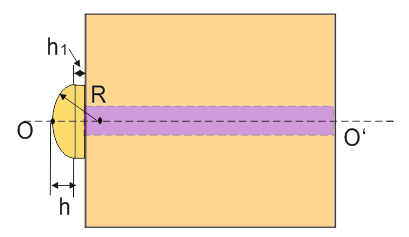
\includegraphics[width=0.7\textwidth]{bilder/lensed_waveguide_neck}
\caption{Schema of a lensed buried waveguide with a 'neck'.}
\label{fig:lensed_waveguide_neck}
\end{figure}
